\chapter{Diffusion Models}

In this chapter, we introduce the Diffusion Model, a family of generative models that have proven to be a valuable framework for novel image generation, text-to-image, text-to-video, and practical applications such as molecular graph modeling and medical image reconstruction \citep{sohldickstein2015deep, ramesh2021zeroshot,rombach2022highresolution,ho2020denoising,singer2022makeavideo,jing2023torsional,song2020denoising}. Proving to be a useful tool and keep this kind of model to be an active research line in the last few years \citep{yang2024diffusion}. \\

\noindent We will review the formulation proposed in the work titled \textit{Denoising Diffusion Probabilistic Models} \cite{ho2020denoising}, or DDPM for short. The primary motivation for basing the discussion of diffusion models on this work is to understand how the pretrained model that this work is based on was trained. In addition, it serves as a framework to understand subsequent improvements and enhancements without significant modifications to the primary ingredients of the recipe. Furthermore, it has a deep connection with theoretical work of score-based generative models \citep{song2020generative, song2020improved, song2021scorebased} and Variational Autoencoders \citep{luo2022understanding}.

\section{Denoising Diffusion Probabilistic Models}

The key idea in Denoising Diffusion Probabilistic Models (DDPM) is to learn a mapping from a complex data distribution to a simple prior distribution, such as a Gaussian. This is achieved by successively corrupting the data with noise, transforming observations of the complex distribution into observations of the simple one. Concurrently, a model is trained to denoise the sequence of noisy observations and recover the original data.\\

\begin{figure}[ht]
    \centering
    \includegraphics[scale=0.22]{ch2-diffusion-models/fwd_noise.png}
    \captionsetup{width=\textwidth} % set the width of the caption
    \caption{Grogu (aka Baby Yoda) joins with the Force through a forward process.}
    \label{fig:fwd-process-grogu}
\end{figure}
  
\noindent Concretely, a forward process which starts from the raw image $\mathrm{x}_{0}$ creates a sequence of intermediate steps between $\mathrm{x}_{1}$ and $\mathrm{x}_{T-1}$, also known as latent states, which are noise perturbations in some degree of the original image's structure as shown in Figure~\ref{fig:fwd-process-grogu}. At the end of the sequence $T$---\textit{if the sequence is infinitely large}---the image is ultimately converted into an isotropic Gaussian noise $p(\mathrm{x}_{T})\sim \mathcal{N}(\mathrm{0}, \mathrm{I})$\footnote{Isotropic is a fancy word for ``equal shape'', and in this context means that the direction of the covariance matrix is all equal.}.\\

\noindent The authors model this forward process $q(\mathrm{x}_{1}\dots\mathrm{x}_{T}\mid\mathrm{x}_{0})$ as a Markov chain, and it follows a transition normal distribution without learnable parameters (aka kernel). 
\begin{align}\label{eqn:forward-process}
q(\mathbf{x}_{1:T}\mid\mathrm{x}_0) &= \prod_{t=1}^{T}q(\mathrm{x}_t\mid\mathrm{x}_{t-1})
\\
q(\mathrm{x}_t\mid\mathrm{x}_{t-1}) &= \mathcal{N}(\mathrm{x}_t;\sqrt{1-\beta_{t}}~\mathrm{x}_{t-1},~ \beta_{t}\mathrm{I})
\end{align}
A deterministic noise scheduler is known beforehand and provides the
amount of noise $\beta_{t}$ for any timestep $t$ of the Markov chain to
generate $\mathrm{x}_{t}$ . How do we think about the latent space? The scale-location transformation\footnote{A quick recap about normal distributions: if $Z$ is a standard normal random variable and $X=\mu + \sigma Z$, then $X$, is a normal random variable with mean $\mu$ and variance $\sigma^2$, i.e., $X\sim\mathcal{N}(\mu, \sigma^2)$.} of $q(\mathrm{x}_{t}\mid\mathrm{x}_{t-1})\sim\mathcal{N}(\mathrm{x}_{t}; \sqrt{1-\beta_{t}} \mathrm{x}_{t-1}, \beta_{t}I)$ allows us to sample the \textcolor{orange}{current latent state $\mathrm{x}_{t}$ as a mixture} of the 
\textcolor{violet}{perturbation injected from noise} $\epsilon_{t-1}$ and \textcolor{teal}{the remaning structure
of the data} from the previous latent state $\mathrm{x}_{t-1}$.

%\textcolor{violet}{how much perturbation inject} from noise $\epsilon_{t-1}$, and \textcolor{teal}{the rest of what left of the image's structure} from the previous latent space $\mathrm{x}_{t-1}$:
\begin{equation}\label{eqn:scale-location-transformation}
    \textcolor{orange}{\mathrm{x}_{t}} = \textcolor{teal}{\sqrt{1-\beta_{t}}}~ \mathrm{x}_{t-1} + \textcolor{violet}{\sqrt{\beta_{t}}}~\mathrm{\epsilon}_{t-1}
\end{equation}
At the same time, there is a backward process---\textit{another Markov chain but in this case in the reverse timestep direction and with a learnable transition kernel}---model by $p_{\theta}(\mathrm{x}_{T:0})$. Specifically, 
the backward process takes the following form:
\begin{align}\label{eqn:backward-process}
    p_{\theta}(\mathrm{x}_{T:0}) &= p(\mathrm{x}_{T})\prod_{t=1}^{T}p_{\theta}(\mathrm{x}_{t-1}\mid\mathrm{x}_{t})
    \\
    p_{\theta}(\mathrm{x}_{t-1}\mid\mathrm{x_{t}}) &= \mathcal{N}(\mathrm{x}_{t-1};~\mu_{\theta}(\mathrm{x}_{t}, t),~\Sigma_{\theta}(\mathrm{x}_{t}, t))
\end{align}
We know that $p(\mathrm{x}_{T})$ is a standard normal distribution when $\beta_{T}\approx 1$ in Equation~\ref{eqn:scale-location-transformation}. Additionally, as we will see in the following sections, there are design options for learning the parameters of the kernel mentioned above. However, in most cases where the data distribution is complex, such as with images or audio, the kernel is parameterized by deep neural networks.\\

\section{Recursive Reparameterization Trick}\label{sec:reparameterization-trick}

% https://stats.stackexchange.com/questions/199605/how-does-the-reparameterization-trick-for-vaes-work-and-why-is-it-important
% https://web.archive.org/web/20160418040123/http://dpkingma.com/wordpress/wp-content/uploads/2015/12/talk_nips_workshop_2015.pdf
The \textit{reparameterization trick} originally appears in the work that introduce the Variational Autoencoder (VAE) model \cite{kingma2013auto} and is also used in the diffusion framework with some modifications. The main goal in the VAE context is to remove the stochasticity of a node variable that depends on parameters from the distribution, \href{https://web.archive.org/web/20160418040123/http://dpkingma.com/wordpress/wp-content/uploads/2015/12/talk_nips_workshop_2015.pdf}{leaving the stochastic part as the noise instantiated in a separate node}. As simple as it appears, this trick makes it possible to create a computational graph to properly backpropagate with automatic differentiation frameworks such as PyTorch or JAX, and update the parameters during training. Nevertheless, in the diffusion context, we will
see that a \textit{recursive} application of the reparameterization trick achieve more than just enabling backpropagation. \\

\noindent Let $\alpha_{t}=1 - \beta_{t}$ and $\bar{\alpha}_{t}=\prod_{i=1}^{t}\alpha_{i}$. Now we proceed to unwind the $t$ index until $t=0$ in Equation~\ref{eqn:scale-location-transformation}, we ended up with a reparametrization of $q(\mathrm{x}_{t}\mid\mathrm{x}_{t-1})$ in terms of $\mathrm{x}_{0}$, and it is possible to sample from it by scaling the normal standard distribution $\sim \mathcal{N}(0, \sigma^2)$ accordingly its parameters:
\begin{equation}\label{eqn:reparameterization-trick}
    \begin{split}
            \mathrm{x}_{t} & = \sqrt{\alpha_{t}}~\mathrm{x}_{t-1} + \sqrt{1-\alpha_{t}}~\epsilon_{t-1} \\
             & = \sqrt{\alpha_{t}}~(\sqrt{\alpha_{t-1}}~\mathrm{x}_{t-2} + \sqrt{1 - \alpha_{t-1}}~\epsilon_{t-2}) + \sqrt{1-\alpha_{t}}~\epsilon_{t-1} \\
             &= \sqrt{\alpha_{t}~\alpha_{t-1}}~\mathrm{x}_{t-2} + \textcolor{orange}{\sqrt{\alpha_{t} - \alpha_{t}~\alpha_{t-1}}~\epsilon_{t-2} + \sqrt{1-\alpha_{t}}~\epsilon_{t-1}} \\
             &= \sqrt{\alpha_{t}~\alpha_{t-1}}~\mathrm{x}_{t-2} + \textcolor{orange}{\sqrt{1 - \alpha_{t}~\alpha_{t-1}}~\bar{\epsilon}_{t-2}} \\
             &= \dots \\
             &= \sqrt{\alpha_{t}~\alpha_{t-1}\dots\alpha_{0}}~\mathrm{x}_{0} + \sqrt{1 - \alpha_{t}~\alpha_{t-1}\dots\alpha_{0}}~\bar{\epsilon}_{0} \\
             &= \sqrt{\prod_{i=1}^{t}\alpha_{i}}~\mathrm{x}_{0} + \sqrt{1 - \prod_{i=1}^{t}\alpha_{i}}~\bar{\epsilon}_{0} \\
             &= \sqrt{\bar{\alpha}_{t}}~\mathrm{x}_{0} + \sqrt{1 - \bar{\alpha}_
             {t}}~\bar{\epsilon}_{0} 
    \end{split}
\end{equation}
Technically, what happens in the above derivation is that the choice of a Gaussian transition kernel $q(\mathrm{x}_{t}\mid\mathrm{x}_{t-1})$ allows us to
\textcolor{orange}{group pairs of Gaussians into a single one, remaining a Gaussian distribution, by just summing up their means and variances}.  By repeteadly aplying this property, we end up marginilizing the joint distribution in Equation~\ref{eqn:forward-process} to obtain an analytical form of $q(\mathrm{x}_{t}\mid \mathrm{x}_{0})$ for all timesteps $t\in\{0, 1, \dots, T\}$ \shortcite{sohldickstein2015deep}. 
\begin{equation}\label{eqn:marginilize_q_xt_on_x0}
    q(\mathrm{x}_{t}\mid \mathrm{x}_{0}) = \mathcal{N}(\mathrm{x}_{t};\sqrt{\bar{\alpha}_{t}}~\mathrm{x}_{0}, (1-\bar{\alpha}_{t})\mathrm{I})
\end{equation}
The remarkable consequence of having a closed form is the ability to sample from $\mathrm{x}_{0}\rightarrow \mathrm{x}_{t}$ without explicitly passing through intermediate steps $\mathrm{x}_{1}, \dots, \mathrm{x}_{t-1}$. Therefore, we can go from $\mathrm{x}_{0}$ to any arbitrary $t$ in just one evaluation---\textit{since $\bar{\alpha}$ is known in advance given the noise scheduler}---making the whole DDPM framework computationally feasible.

\section{Optimization}\label{sec:optimization-ddpm}

We can sample a batch of inputs from the data distribution $\mathrm{x}_{0}\sim q(\mathrm{x}_{0})$, such as images, and corrupt them with noise $\epsilon\sim\mathcal{N}(0, I)$ according to a scale factor $\bar{\alpha}_{t}$, obtaining the latent states from the timesteps $t\sim\mathcal{U}[1, T]$ using Equation~\ref{eqn:reparameterization-trick}. For training DDPM, the authors choose only to learn the mean of the backward kernel and use a time-dependent constant variance $\sigma_{t}^{2}$ for all $t$\footnote{The authors add a diagonal learnable variance $\Sigma_{\theta}(\mathrm{x}_{t})$ but they obtained unstable training and poor sample quality.}. Rather than learning the mean of the backward kernel directly, they achieve this indirectly by predicting the noise perturbation $\epsilon_{\theta}^{(t)}(\mathrm{x}_{t})$. The training objective defined in DDPM is the following:
\begin{equation}\label{eqn:ho-eq12}
    \mathbb{E}_{t\sim\mathcal{U}[1, T], \mathrm{x}_{0}\sim q(\mathrm{x}_{0}), \epsilon\sim\mathcal{N}(0, \mathrm{I})}  \big[\lambda(t) ~ \|\epsilon - \epsilon_{\theta}^{(t)}(\mathrm{x}_{t}) \|^{2} \big]
\end{equation}
Where $\lambda(t)= \beta_{t}^{2} / 2\sigma_{t}^{2}\alpha_{t}(1-\bar{\alpha}_{t})$. Empirical results shows that it is possible to discard $\lambda(t)$ without affecting sample quality, resulting in the following simplified objective:
\begin{equation}\label{eqn:ho-eq14}
    \mathbb{E}_{t\sim\mathcal{U}[1, T], \mathrm{x}_{0}\sim q(\mathrm{x}_{0}), \epsilon\sim\mathcal{N}(0, \mathrm{I})} \big[\| \epsilon - \epsilon_{\theta}^{(t)}(\sqrt{\bar{\alpha}_{t}}~\mathrm{x}_{0} + \sqrt{1-\bar{\alpha}_{t}}~\epsilon) ||^{2} \big]
\end{equation}
The simplified loss is just a mean squared error, and a description of the
training procedure is shown in Algorithm 1. Notice that the backward process $p_{\theta}(\mathrm{x}_{1:T})$ is parameterized by a collection of $T$ denoiser functions $\epsilon_{\theta}^{(t)}$ with learnable parameters $\theta^{(t)}$.
\begin{figure}[ht]\label{alg:ddpm-training-sampling}
    \begin{minipage}{0.45\textwidth}
    \begin{algorithm}[H]
        \caption{DDPM Training}
        \begin{algorithmic}
            \STATE \textbf{repeat}
            \STATE  ~~~~$\mathrm{x}_{0}\sim q(\mathrm{x_{0}})$
            \STATE  ~~~~$t\sim \mathcal{U}(1, T)$
            \STATE  ~~~~$\epsilon\sim \mathcal{N}(0, \mathrm{I})$
            \STATE  ~~~~Take gradient descent step on
            \STATE  $~~~~~~~~\nabla_{\theta}\|\epsilon - \epsilon_{\theta}^{(t)}(\sqrt{\bar{\alpha}_{t}}\mathrm{x}_{0} + \sqrt{1-\bar{\alpha}_{t}}\epsilon) \|^{2}$
            \STATE \textbf{until} converged
        \end{algorithmic}
    \end{algorithm}
    \end{minipage}
    \hspace{0.25cm}
    %\hfill
    \begin{minipage}{0.45\textwidth}
    \begin{algorithm}[H]
        \caption{DDPM Sampling}
        \begin{algorithmic}
        \STATE  $\mathrm{x}_{T}\sim\mathcal{N}(\mathrm{0}, \mathrm{I})$
        \FOR{$t=T, \dots, 1$}
            \STATE $\mathrm{z}\sim\mathcal{N}(0, \mathrm{I})$
            \STATE $\mathrm{x}_{t-1}=\frac{1}{\sqrt{\alpha_{t}}} \bigg(\mathrm{x}_{t} - \frac{1-\alpha_{t}}{\sqrt{1-\bar{\alpha}_{t}}}\epsilon_{\theta}^{(t)}(\mathrm{x}_{t})\bigg) + \sigma_{t}\mathrm{z}$
        \ENDFOR
        \STATE \textbf{return} $\mathrm{x}_{0}$
        \end{algorithmic}
    \end{algorithm}
    \end{minipage}
    \end{figure}


\noindent In the next sections we will justify the use of the above loss function and the training algorithm in the context of the Variational Lower Bound (VLB).

\subsection{Variational Lower Bound}\label{sec:variational-lower-bound}

    %https://chrisorm.github.io/VI-ELBO.html
    %esto se puede derivar desde la divergencia de Kullback-Leibler
    % o usando Jensen Inequality. En paper summary se ocupa KL, se podría
    % mostrar esa conciliaición...

DDPM are training by optimizing the Variational Lower Bound (VLB)
on the negative log-likelihood of the learnable distribution.
\begin{equation}\label{eqn:ELBO1}
    \begin{split} 
        -\log p_{\theta}(\mathrm{x}_{0}) &= -\log\int p_{\theta}(\mathrm{x}_{0:T}) d\mathrm{x}_{1:T} \\
        &= -\log \int \frac{p_{\theta}(\mathrm{x}_{0:T})q(\mathrm{x}_{1:T}\mid\mathrm{x}_{0})}{q(\mathrm{x}_{1:T}\mid\mathrm{x}_{0})}d\mathrm{x}_{1:T} \\
        &= - \log \mathbb{E}_{q(\mathrm{x}_{1:T}\mid\mathrm{x}_0)} \bigg[\frac{p_{\theta}(\mathrm{x}_{0:T})}{q(\mathrm{x}_{1:T}\mid\mathrm{x}_{0})} \bigg] \\
        % -\log p_{\theta}(\mathrm{x}_{0}) 
        & \leq \mathbb{E}_{q(\mathrm{x}_{1:T}\mid\mathrm{x}_{0})}\bigg[-\log \frac{p_{\theta}(\mathrm{x}_{0:T})}{q(\mathrm{x}_{1:T}\mid\mathrm{x}_{0})}\bigg] \\
        &\leq \mathbb{E}_{q(\mathrm{x}_{1:T}\mid\mathrm{x}_{0})}\bigg[-\log p(\mathrm{x}_{T}) - \sum_{t\geq 1}^{T} \log\frac{p_{\theta}(\mathrm{x}_{t-1}\mid\mathrm{x}_{t})}{q(\mathrm{x}_{t}\mid\mathrm{x}_{t-1})} \bigg] \\
        L &:= \mathbb{E}_{q(\mathrm{x}_{1:T}\mid\mathrm{x}_{0})}\bigg[-\log p(\mathrm{x}_{T}) - \sum_{t>1}^{T} \log \frac{p_{\theta}(\mathrm{x}_{t-1}\mid\mathrm{x}_{t})}{q(\mathrm{x}_{t}\mid\mathrm{x}_{t-1})}-\log\frac{p_{\theta}(\mathrm{x}_{0}\mid\mathrm{x}_{1})}{q(\mathrm{x}_{1}\mid\mathrm{x}_{0})}\bigg]
    \end{split}
\end{equation}

\noindent The first step in Equation~\ref{eqn:ELBO1} is to apply the definition of the negative log-likelihood and integrate out $\mathrm{x}_{1:T}$ from the
joint distribution $p_{\theta}(\mathrm{x}_{0:T})$. Then, we multiply by 1,
introducing $q(\mathrm{x}_{1:T}\mid\mathrm{x}_{0})/q(\mathrm{x}_{1:T}\mid\mathrm{x}_{0})$, and use the expectation operator. We use the Jensen's inequality to bound the negative log-likelihood by the expectation of the negative log-likelihood. \\

\noindent In the last steps, we decompose the expectation into the sum of the negative log-likelihood of the forward and backward processes, applying the Markov property to both. Notice the last term $\mathrm{x}_{T}$ is decouple from $p_{\theta}(\mathrm{x}_{0:T})$ because, for a sufficiently large sequence $T\gg$, we know that we will get a final state described by $\mathcal{N}(0, \sigma^2\mathrm{I})$. Therefore, we keep it separate in the same way as the first transition step $\mathrm{x}_{0}\mid\mathrm{x_{1}}$ and $\mathrm{x}_1\mid\mathrm{x}_0$ that involves the raw data $\mathrm{x}_{0}$ in each process.\\
    
\noindent The training objective is derived from the VLB, following the methods outlined in the relevant literature \cite{sohldickstein2015deep}\cite{ho2020denoising}\cite{luo2022understanding}. Due to space constraints, we refer to $\mathbb{E}_{q(\mathrm{x}_{1:T}\mid\mathrm{x}_{0})}$ as $\mathbb{E}_{q}$.

\begin{equation}\label{eqn:ELBO2}
    \begin{split}
        L_{\text{\scriptsize{\text{VLB}}}} & = \mathbb{E}_{q}\bigg[-\log p(\mathrm{x}_{T}) - \sum_{t>1}^{T} \log \frac{p_{\theta}(\mathrm{x}_{t-1}\mid\mathrm{x}_{t})}{q(\mathrm{x}_{t}\mid\mathrm{x}_{t-1})}-\log\frac{p_{\theta}(\mathrm{x}_{0}\mid\mathrm{x}_{1})}{q(\mathrm{x}_{1}\mid\mathrm{x}_{0})}\bigg] \\
        & = \mathbb{E}_{q}\bigg[-\log p(\mathrm{x}_{T}) - \sum_{t>1}^{T} \log \frac{p_{\theta}(\mathrm{x}_{t-1}\mid\mathrm{x}_{t})}{\textcolor{teal}{q(\mathrm{x}_{t-1}\mid\mathrm{x}_{t},~\mathrm{x}_{0})}}\frac{\textcolor{Magenta}{q(\mathrm{x}_{t-1}\mid\mathrm{x}_{0})}}{\textcolor{violet}{q(\mathrm{x}_{t}\mid\mathrm{x}_{0})}}-\log\frac{p_{\theta}(\mathrm{x}_{0}\mid\mathrm{x}_{1})}{q(\mathrm{x}_{1}\mid\mathrm{x}_{0})}\bigg] \\
        & = \mathbb{E}_{q}\bigg[-\log p(\mathrm{x}_{T}) - \sum_{t>1}^{T} \log \frac{p_{\theta}(\mathrm{x}_{t-1}\mid\mathrm{x}_{t})}{\textcolor{teal}{q(\mathrm{x}_{t-1}\mid\mathrm{x}_{t},~\mathrm{x}_{0})}} -\sum_{t>1}^{T}\log \frac{\textcolor{Magenta}{q(\mathrm{x}_{t-1}\mid\mathrm{x}_{0})}}{\textcolor{violet}{q(\mathrm{x}_{t}\mid\mathrm{x}_{0})}}-\log\frac{p_{\theta}(\mathrm{x}_{0}\mid\mathrm{x}_{1})}{q(\mathrm{x}_{1}\mid\mathrm{x}_{0})}\bigg] \\
        & = \mathbb{E}_{q}\bigg[-\log p(\mathrm{x}_{T}) - \sum_{t>1}^{T} \log \frac{p_{\theta}(\mathrm{x}_{t-1}\mid\mathrm{x}_{t})}{\textcolor{teal}{q(\mathrm{x}_{t-1}\mid\mathrm{x}_{t}, \mathrm{x}_{0})}}- \log\frac{\textcolor{orange}{q(\mathrm{x}_{1}\mid\mathrm{x}_{0})}}{\textcolor{violet}{q(\mathrm{x}_{T}\mid\mathrm{x}_{0})}} -\log\frac{p_{\theta}(\mathrm{x}_{0}\mid\mathrm{x}_{1})}{q(\mathrm{x}_{1}\mid\mathrm{x}_{0})}\bigg] \\
        & = \mathbb{E}_{q}\bigg[-\log p(\mathrm{x}_{T}) - \sum_{t>1}^{T} \log \frac{p_{\theta}(\mathrm{x}_{t-1}\mid\mathrm{x}_{t})}{\textcolor{teal}{q(\mathrm{x}_{t-1}\mid\mathrm{x}_{t}, \mathrm{x}_{0})}}- \log\textcolor{orange}{q(\mathrm{x}_{1}\mid\mathrm{x}_{0})} + \log \textcolor{violet}{q(\mathrm{x}_{T}\mid\mathrm{x}_{0})} -\log\frac{p_{\theta}(\mathrm{x}_{0}\mid\mathrm{x}_{1})}{q(\mathrm{x}_{1}\mid\mathrm{x}_{0})}\bigg] \\
        & = \mathbb{E}_{q}\bigg[-\big(\log p(\mathrm{x}_{T}) - \log \textcolor{violet}{q(\mathrm{x}_{T}\mid\mathrm{x}_{0})}\big) - \sum_{t>1}^{T} \log \frac{p_{\theta}(\mathrm{x}_{t-1}\mid\mathrm{x}_{t})}{\textcolor{teal}{q(\mathrm{x}_{t-1}\mid\mathrm{x}_{t}, \mathrm{x}_{0})}} - \big( \log\textcolor{orange}{q(\mathrm{x}_{1}\mid\mathrm{x}_{0})}  +\log\frac{p_{\theta}(\mathrm{x}_{0}\mid\mathrm{x}_{1})}{q(\mathrm{x}_{1}\mid\mathrm{x}_{0})}\big)\bigg]  \\ 
        & = \mathbb{E}_{q}\bigg[-\log \frac{p(\mathrm{x}_{T})}{\textcolor{violet}{q(\mathrm{x}_{T}\mid\mathrm{x}_{0})}} - \sum_{t>1}^{T} \log \frac{p_{\theta}(\mathrm{x}_{t-1}\mid\mathrm{x}_{t})}{\textcolor{teal}{q(\mathrm{x}_{t-1}\mid\mathrm{x}_{t}, \mathrm{x}_{0})}} -  \log p_{\theta}(\mathrm{x}_{0}\mid\mathrm{x}_{1})\bigg]  \\
        & = \mathbb{E}_{q(\mathrm{x}_{1:T}\mid\mathrm{x}_{0})}\bigg[\underbrace{D_{\text{\scriptsize{KL}}}\big(\textcolor{violet}{q(\mathrm{x}_{T}\mid\mathrm{x}_{0})} ||~p(\mathrm{x}_{T}) \big)}_{L_{T}} + \sum_{t>1}^{T} \underbrace{D_{\text{\scriptsize{KL}}}\big( \textcolor{teal}{q(\mathrm{x}_{t-1}\mid\mathrm{x}_{t}, \mathrm{x}_{0})}||~p_{\theta}(\mathrm{x}_{t-1}\mid\mathrm{x}_{t}) \big)}_{L_{t-1}} -  \underbrace{\log p_{\theta}(\mathrm{x}_{0}\mid\mathrm{x}_{1})}_{L_{0}} \bigg]
    \end{split}
\end{equation}

\noindent The key points from the above derivation are as follows: 
\begin{enumerate}
    \item Isolating  $\log q(\mathrm{x}_{t}\mid\mathrm{x}_{0})$ with $\log p(\mathrm{x}_{T})$ because both are invariant by the learning process.
    \item Reversing $q(\mathrm{x}_{t}\mid\mathrm{x}_{t-1})$ by $q(\mathrm{x}_{t-1}\mid\mathrm{x}_{t}, \mathrm{x}_{0})$ (bayes theorem) in step 2. 
    % \ca{completar este paso...}. 
    \item The first two terms at the end of Equation~\ref{eqn:ELBO2} appear due to the definition of the Kullback-Leibler divergence. 
\end{enumerate}
    
\noindent In summary, the variational lower bound loss is a sum of terms that result from the reverse diffusion process $L_{\text{\scriptsize{\text{VLB}}}}=L_{T} + L_{T-1} + \dots + L_{0}$. The final term $L_{T}$ can be discarded because
it is constant, given that $q$ has not learnable parameters and $\mathrm{x}_{T}$ follows a standard normal distribution. The remaining terms are the denoising matching terms, which are crucial in the loss function because their number depends on the length of diffusion chain $T$ (e.g. $T=1000$ in DDPM).\\

\subsection{Denoising Matching Term}

The model's goal is to minimize the discrepancy, measured by the Kullback-Leibler divergence, between the posterior of the encoder---\textit{which tells us how to remove the real noise}---and the decoder, which predicts how to ``reverse'' the processes and has learnable parameters $\theta$. Therefore, the loss consists of a sum of denoising matching terms across the diffusion sequence, as shown in Figure~\ref{fig:ddpm-denoising-term}. \\

\begin{figure}[t]
  \centering
  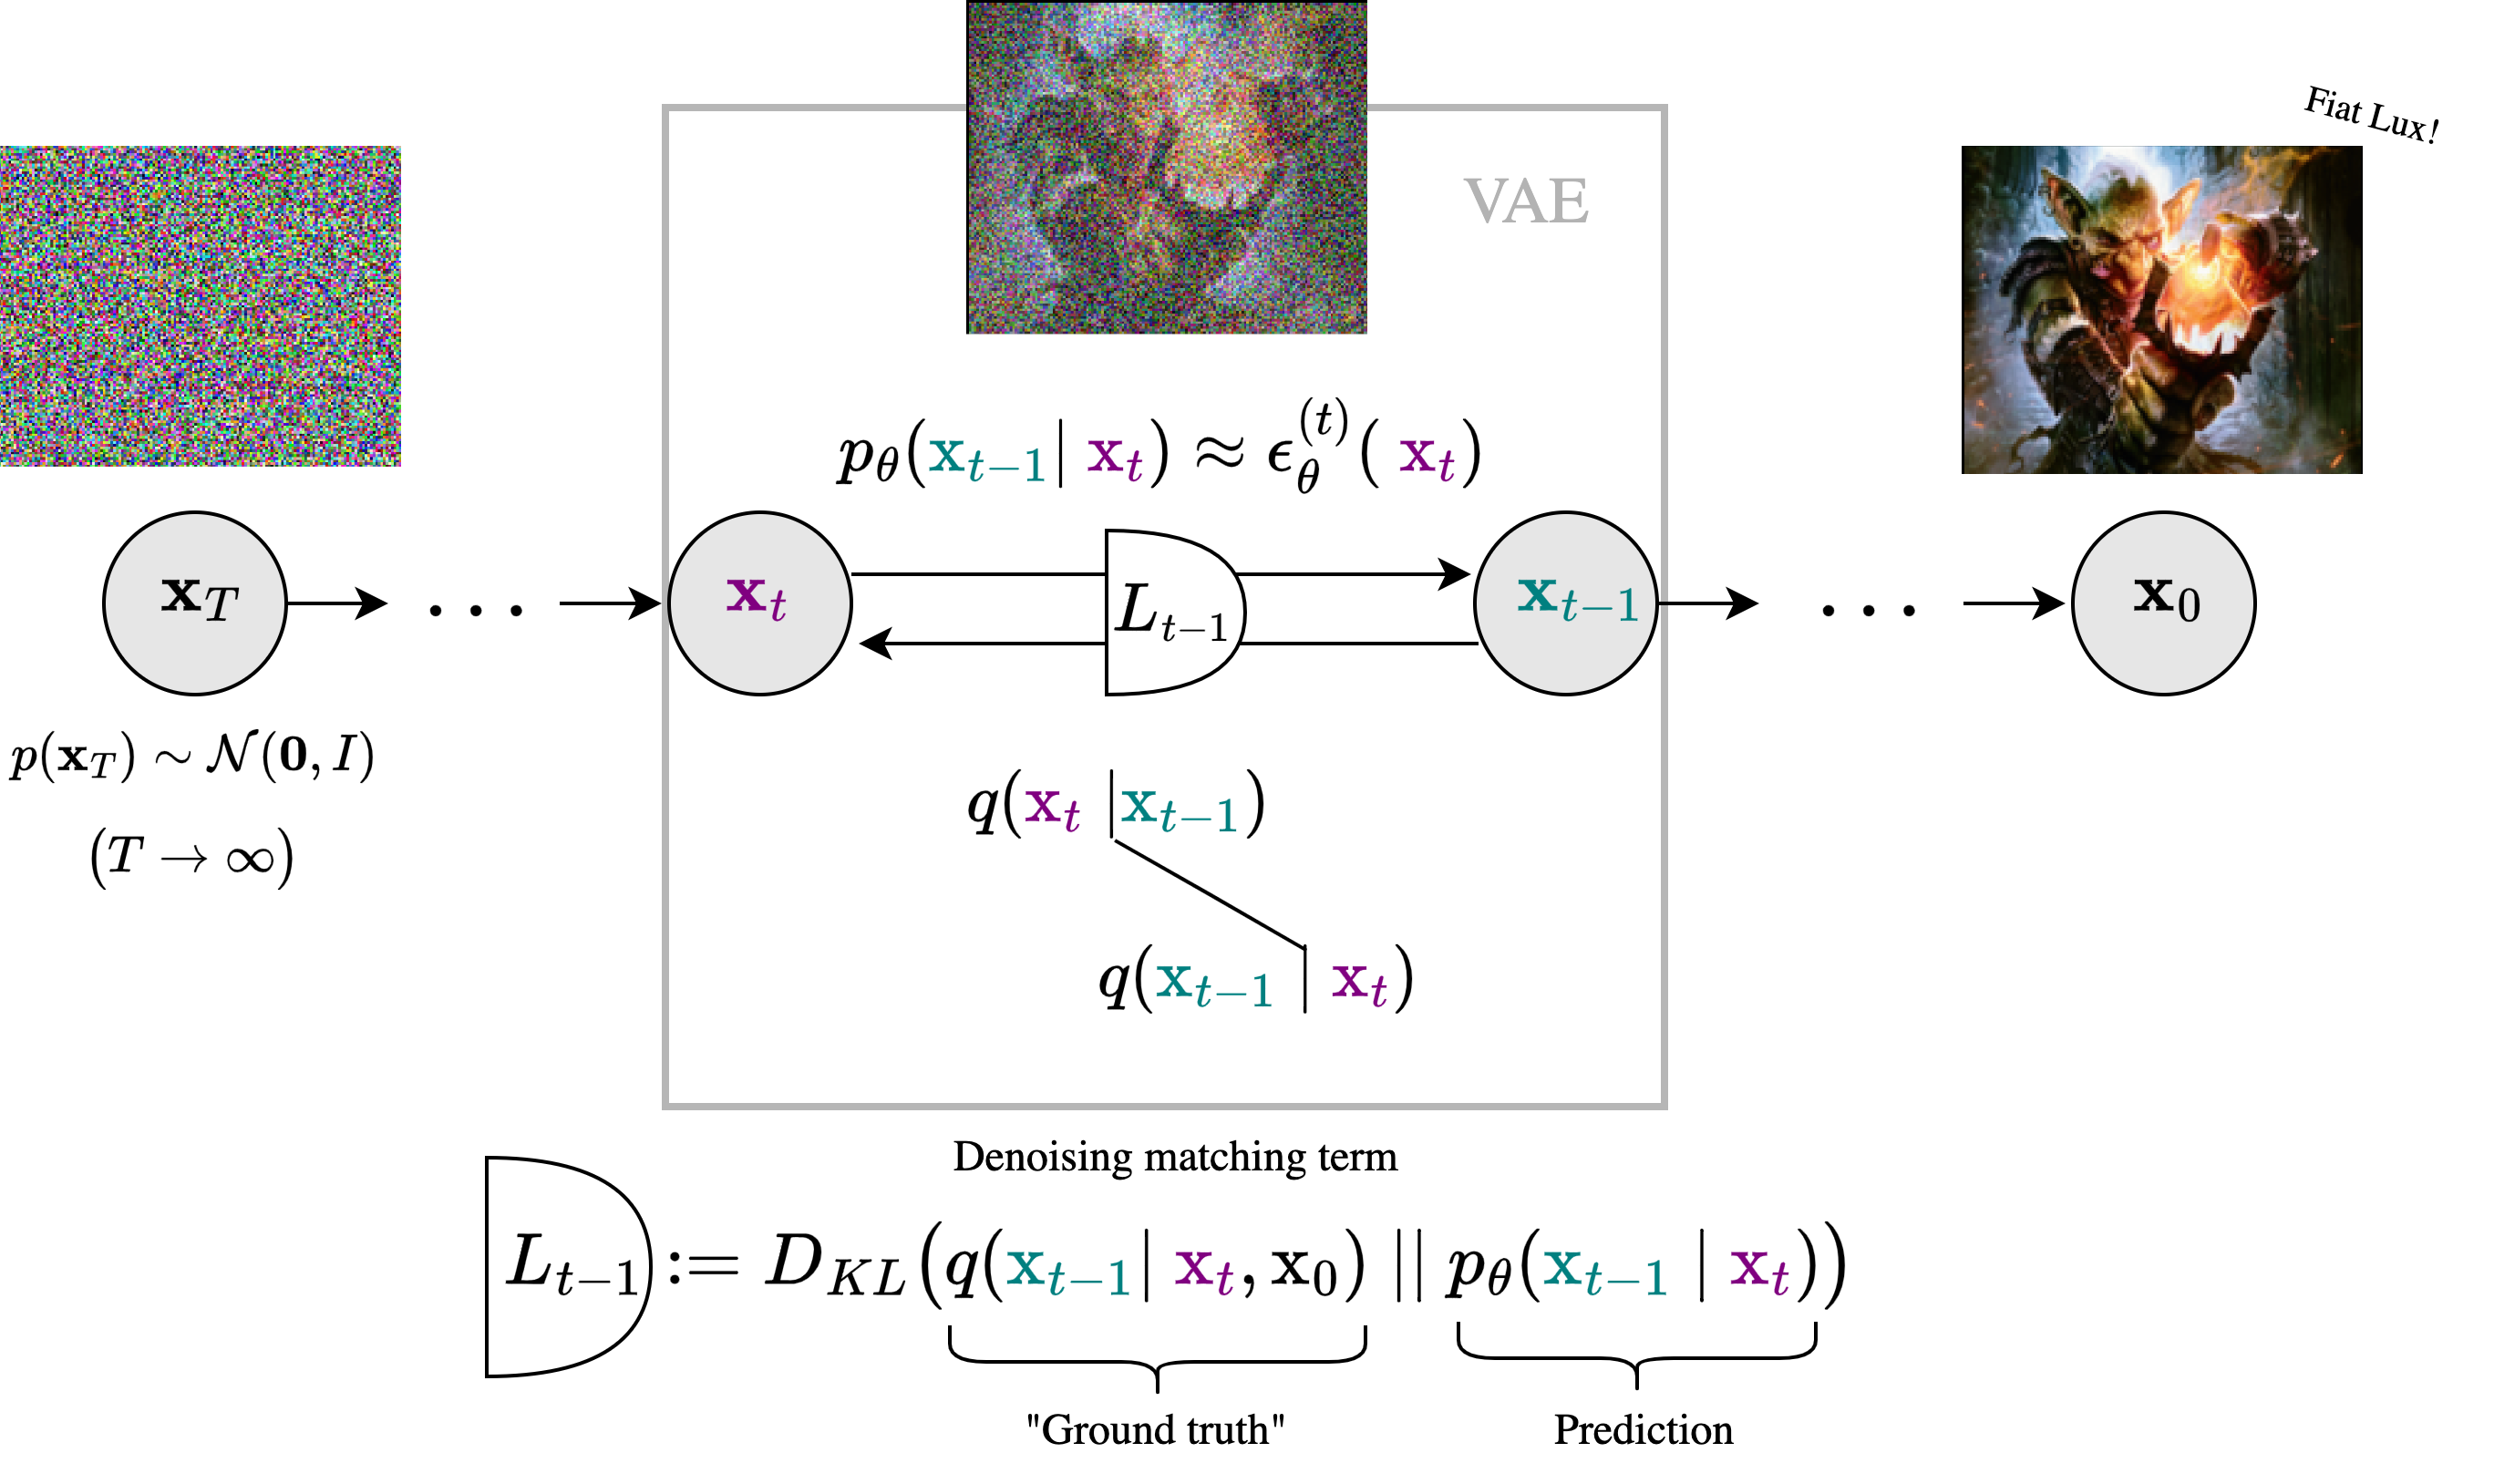
\includegraphics[scale=0.8]{ch2-diffusion-models/DDPM-HMVAE-simple.png}
  \captionsetup{width=\textwidth} % set the width of the caption
  \caption{\textbf{Denoising matching term in action.} \textbf{Left:} $\mathrm{x}_{T}$ is a pure Gaussian noise. \textbf{Middle:} Transition from a noisy intermediate state to a less noisy one; the denoising matching term forces $p_{\theta}$ to be similar to the posterior forward kernel $q(\mathrm{x}_{t-1}\mid \mathrm{x}_{t})$. \textbf{Right:} $\mathrm{x}_{0}$ the input image during training.}
  \label{fig:ddpm-denoising-term}
\end{figure}

\noindent However, reversing the diffusion process $q(\mathrm{x}_{t-1}\mid\mathrm{x}_{t})$ is intractable because it requires the entire dataset to compute it. We can make it tractable by conditioning on $\mathrm{x}_{0}$, leading to the following expression\footnote{(See \citep{weng2021diffusion} for a detailed derivation)}:

\begin{align}\label{eqn:reverse-forward-process}
    q(\mathrm{x}_{t-1}\mid\mathrm{x}_{t}, \mathrm{x}_{0}) &= \mathcal{N}(\mathrm{x}_{t-1};~\tilde{\mu}_{t}(\mathrm{x}_{t}), \tilde{\beta}_{t}I) \\
    \tilde{\mu_{t}}(\mathrm{x}_{t}) &= \frac{1}{\sqrt{\alpha_{t}}}\big(\mathrm{x}_{t} - \frac{1 - \alpha_{t}}{\sqrt{1 - \bar{\alpha}}_{t}}\epsilon_{t}\big) \\
    \tilde{\beta}_{t} &= \frac{1-\bar{\alpha}_{t-1}}{1-\bar{\alpha}_{t}}\beta_{t}
\end{align}

\noindent The parameterization in the backward process will be to match
$\tilde{\mu}_{t}$, 

\begin{align}\label{eqn:backward-noise-reparameterization}
    \mu_{\theta}(\mathrm{x}_{t}, t) &= \frac{1}{\sqrt{\alpha_{t}}}\big(\mathrm{x}_{t} - \frac{1-\alpha_{t}}{\sqrt{1-\bar{\alpha}_{t}}}\epsilon_{\theta}^{(t)}(\mathrm{x}_{t})\big) \\
    \mathrm{x}_{t-1} &= \mathcal{N}\big(\mathrm{x}_{t-1}; \frac{1}{\sqrt{\alpha_{t}}}\big(\mathrm{x}_{t} - \frac{1-\alpha_{t}}{\sqrt{1-\bar{\alpha}_{t}}}\epsilon_{\theta}(\mathrm{x}_{t}, t)\big), \Sigma_{\theta}(\mathrm{x}_{t}, t)\big)
\end{align}

% \noindent \ca{Conectar con la intro de la sección optimization} Another important aspect is the parameterization of $p_{\theta}$ we can predict directly the latent state $\mathrm{x}_{t-1}$, or indirectly by predicting the noise perturbation $\epsilon_{\theta}$, and then apply the reparameterization trick to get the latent state, given that $\mathrm{x}_{t}$ is known. Moreover,
% in (Ho et al., 2020) \cite{ho2020denoising} they use only the mean as a learnable parameter and the variance is set as $\Sigma_{\theta}(\mathrm{x}_{t}, t)=\sigma_{t}^2I$, a time dependent constant such as $\sigma_{t}^{2}=\beta_{t}$ or $\sigma_{t}^{2}=\tilde{\beta}_{t}$.

\noindent In DDPM show good performance with only learning the mean
and fix the variance using a time dependent constant $\Sigma_{\theta}(\mathrm{x}_{t}, t) = \sigma_{t}^{2}I$. When the authors tried to learn the variance they get poor results and unstable training, that in further studies is it shown how to stabilizie and learn also the variance \citep{nichol2021improved}.

\begin{align}\label{eqn:backward-process-fix-variance}
    p_{\theta}(\mathrm{x}_{t-1}\mid\mathrm{x_{t}}) &= \mathcal{N}(\mathrm{x}_{t-1};~\mu_{\theta}(\mathrm{x}_{t}, t), \sigma_{t}^{2}I)
\end{align}

% Therefore, we have everything to expand the denoising matching term $L_t$ with $1\leq t < T$ terms \ca{Además, emerge de la \href{https://kvfrans.com/deriving-the-kl/}{definición de KL de sumatorias entre dos gaussiano un MSE}.}: \\

% \ca{Mejorar esta parte y dar más hincapie a la VLB compartida}
\noindent Finally, as you can see in Figure~\ref{fig:ddpm-denoising-term}, the denoising matching term within the gray square remarks the VAE loss term. However, there are some differences between the VAE and the DDPM: (i) VAE is optimize in the latent space, while DDPM is optimize in the data space (e.g. CelebaHQ 256x256), (ii) VAE use a kernel that is learnable, while DDPM use a fixed kernel, and (iii) VAE perform a single step of sampling, while DDPM perform a large number of steps, hence is more similar to a hierarchical VAE \citep{luo2022understanding}.\\


\section{Score-based generative models}\label{sec:ddpm-as-score}

% \ca{Ver sección 24.3.2 Denoising score matching (DSM) del libro de tópicos avanzados de Murphy}

In this section, we aim to establish a connection between DDPM and score-based generative models \citep{song2020generative, song2020improved, song2021scorebased}. The purpose is more conceptual than practical concerning the work of this thesis, as the literature on how to condition diffusion models is built on this theoretical perspective, and it is a way to increase the degree of control over diffusion models. \\

\noindent It turns out that the objective of Equation~\ref{eqn:ho-eq12}, derived from the variational lower bound (Section~\ref{sec:variational-lower-bound}) and the reparameterization of predicting $\epsilon_{\theta}^{(t)}$ versus directly the latent states, is equivalent to the objective function of Noise Conditional Score Network (NCSN) \citep{song2020improved}. This is a generative model that seeks to learn the data distribution through the score function. We will briefly contextualize this family of models below. \\

\noindent The score function $s(\mathrm{x}_{0})$ of the data distribution $q(\mathrm{x}_{0})$ is defined as the gradient of the log-likelihood w.r.t $\mathrm{x}_{0}$, i.e. $\nabla_{\mathrm{x}_{0}}\log q(\mathrm{x}_{0})$, and it is invariant to scale changes in the distribution. \\

\noindent First, let's start by model the data distribution $q(\mathrm{x}_{0})$ with $p_{\theta}(\mathrm{x}_{0})$:
\begin{equation}\label{eqn:model-directly-density}
    p_{\theta}(\mathrm{x}_{0}) = \frac{e^{-f_{\theta}(\mathrm{x}_{0})}}{\mathrm{Z}_{\theta}} 
\end{equation}

\noindent $f_{\theta}$ is the unnormalized probabilistic model and $\mathrm{Z}_{\theta}$ is the normalizing constant to ensure that the distribution integrates to 1.  The problem is that computing $\mathrm{Z}_{\theta}$ is intractable for high-dimensional data, but we can avoid this by inducing the score function $s_{\theta}(\mathrm{x}_{0})$ in Equation~\ref{eqn:model-directly-density}: \\

\begin{equation}\label{eqn:score-function}
    \begin{split}
        \log p_{\theta}(\mathrm{x}_{0}) &= -f_{\theta}(\mathrm{x}_{0}) - \log \mathrm{Z}_{\theta}  \\
        \nabla_{\mathrm{x}_{0}}\log p_{\theta}(\mathrm{x}_{0}) &= -\nabla_{\mathrm{x}_{0}} f_{\theta}(\mathrm{x}_{0}) - \cancel{\nabla_{\mathrm{x}_{0}}\log \mathrm{Z}_{\theta}} \\
        s_{\theta}(\mathrm{x}_{0}) &= -\nabla_{\mathrm{x}_{0}} f_{\theta}(\mathrm{x}_{0})
    \end{split}
\end{equation}

% \noindent \textbf{TODO:} Introducción de multiples niveles de ruido $\sigma_{i}$ para lidiar con el manifold problem y obtener estimaciones del score más precisas... \\

\begin{equation}
   \mathbb{E}_{p(\mathrm{x})}\bigg[\| \nabla_{x}\log p(x) - s_{\theta}(x)\|_{2}^{2} \bigg]
\end{equation}

\begin{equation}\label{train-objective-ncsn}
    \sum_{i=1}^{L} \lambda (i) \mathbb{E}_{p_{\sigma_{i}}(\mathrm{x})} [ \nabla_{\mathrm{x}} \log p_{\sigma_{i}}(\mathrm{x}) - s_{\theta}(\mathrm{x, i}) ]
\end{equation}

% \noindent \textbf{TODO: Crear transición smooth en este párrafo...} \ca{paper SDE unifican los approaches como dos casos especiales} 

\noindent By generalizing the number of noise scales to infinity, we further proved that score-based generative models and diffusion probabilistic models can both be viewed as discretizations to stochastic differential equations determined by score functions. This work bridges both score-based generative modeling and diffusion probabilistic modeling into a unified framework. \\

\noindent In DDPM work \cite{ho2020denoising}, the authors establish that the denoiser function $\epsilon_{\theta}^{(t)}$ is equivalent to the score function $s_{\theta}(\mathrm{x}_{t})$ in the score-based generative models. The following equation shows the relationship between the score function and the denoiser function, where is derive by combining Tweedie's formula and the reparameterization trick \cite{luo2022understanding}:

\begin{equation}\label{eqn:ddpm-to-score}
    \begin{split}
        \nabla_{\mathrm{x}_{t}}\log p_{\theta}(\mathrm{x}_{t}) &= - \frac{1}{\sqrt{1-\bar{\alpha}_{t}}}\epsilon^{(t)}_{\theta}(\mathrm{x}_{t}) \\
        \epsilon_{\theta}^{(t)}(\mathrm{x}_{t}) &= -\sqrt{1-\bar{\alpha}_{t}}\nabla_{\mathrm{x}_{t}}\log p_{\theta}(\mathrm{x}_{t})
    \end{split}
\end{equation}


\section{Sampling}\label{sec:sampling}

%\ca{\textbf{Importante:} la reparametrización que aparece en el algoritmo de
%sampling, la derivación para llegar a esta se encuentra en \href{https://lilianweng.github.io/posts/2021-07-11-diffusion-models/}{post de difusion de lilian weng} } \\

%once we have trained the model, $\mathrm{x}_{0}$ is obtained by sampling from the prior $p_{\theta}(\mathrm{x}_{t})\sim\mathcal{n}(0, \mathrm{i})$, and then applying \textit{ancestral sampling} through the reverse markovian process, that is appliying iteratiively the denoiser network until to get the final sample.  the algorithm~2 shows the sampling process in detail. \\

%\noindent notice that ddpm requires training the model with a large number of steps $t$
%to allow the reverse process to be close to a gaussian. in ddpm, the hyperparameter $t$ is set to 1000 steps. one consequence of this is that sample from model is computational expensive because the ancestral sampling obtain the next generation $t-1$ from conditioning in the current state $t$ and requires to progress for every step $t$ sequentially. \\

%\noindent \ca{será necesario la conexión con langevin dynamics?} this is done by langevin dynamics, which is a stochastic process that follows the gradient of the log-likelihood. the langevin dynamics is defined by the following equation:
%\begin{equation}
    %\mathrm{x}_{t-1} = \mathrm{x}_{t} + \epsilon \nabla_{x}\log p(x) + \sqrt{2\epsilon}z_{t}, ~~~~~ t=0,1, \dots, t
%\end{equation}

In diffusion models, sampling is a critical process involving the generation of new samples from a learned distribution. After training a model, sampling starts by drawing a sample from a prior distribution, often a standard Gaussian distribution, $p_{\theta}(\mathrm{x}_{T}) \sim \mathcal{N}(0, \mathrm{I})$. Ancestral sampling is then applied by iteratively using the denoiser network through a reverse Markovian process. This process involves applying the denoiser at each step to progressively refine the sample until the final output, $\mathrm{x}_{0}$, is achieved. The detailed steps of this procedure are outlined in Algorithm 2, which demonstrates how each iteration in the reverse process refines the sample. \\

\noindent The Diffusion Probabilistic Models (DDPM) require a significant number of steps, $T$, to closely approximate a Gaussian distribution in the reverse process. For example, a typical setting might use $T = 1000$ steps. This large number of steps is crucial for achieving high-quality samples but also makes the sampling process computationally expensive. Each step \( t \) in the reverse process depends on the previous state, and thus, the ancestral sampling requires sequential computation from $T$ down to $0$, making the process time-consuming. This is reflected in Algorithm 2, where each step in the reverse process involves computing an update based on the previous state and the model's prediction of noise, $\epsilon_{\theta}^{(t)}$, to iteratively refine the sample. \\

\noindent To address the computational cost, score-based models offer an alternative approach by utilizing the score function of the data distribution. These models directly estimate the gradient of the data distribution, $\nabla_{\mathrm{x}} \log p(\mathrm{x})$, which is used in Langevin dynamics to guide the sampling process. The Langevin update rule,

\begin{equation}
    \mathrm{x}_{t-1} = \mathrm{x}_{t} + \epsilon \nabla_{\mathrm{x}} \log p(\mathrm{x}) + \sqrt{2\epsilon} z_{t},
\end{equation}

\noindent Integrates this gradient information to refine the sample iteratively. While not identical, this method relates to DDPM’s sampling algorithm by leveraging gradient information to enhance the efficiency of the sampling process, potentially reducing the number of required steps and computational expense. \\


    
\section{Condition the model}

So far, we know how to learn indirectly the unconditional probability distribution $p(\mathrm{x})$ via the score function $\nabla_{\mathrm{x}}\log p(\mathrm{x})$, but what can we do to condition $\mathrm{x}$ given a signal $\mathrm{y}$, such as a text prompt, another image, or an audio?\\

\noindent By Bayes' theorem, log operations, and taking the gradient w.r.t. $\mathrm{x}$ we got:

\begin{equation}\label{eqn:bayes-conditional-model}
    \begin{split}
        p(\mathrm{x} \mid \mathrm{y}) &= \frac{p(\mathrm{y} \mid \mathrm{x}) \cdot p(\mathrm{x})}{p(\mathrm{y})}\\
        \implies \log p(\mathrm{x} \mid \mathrm{y}) &= \log p(\mathrm{y} \mid \mathrm{x}) + \log p(\mathrm{x}) - \log p(\mathrm{y}) \\
        \implies \nabla_\mathrm{x} \log p(\mathrm{x} \mid \mathrm{y}) &= \nabla_x \log p(\mathrm{y} \mid \mathrm{x}) + \nabla_\mathrm{x} \log p(\mathrm{x})
    \end{split}
\end{equation}
    
\noindent \textbf{TODO:} Review and cite the following \href{https://sander.ai/2023/08/28/geometry.html}{blog posts} \cite{dieleman2022guidance} and \cite{dieleman2023geometry} about guidance. Se podría describir los términos de la
Ecuación~\ref{eqn:bayes-conditional-model} en base al capítulo de Murphy en
vez de utilizar la referencia en la siguiente sección...


\subsection{Classifier Guidance (CG)}\label{sec:clip-cg}

\textbf{C}lassifier \textbf{G}uidance is a technique to condition the model by using a classifier to guide the sampling process once the diffusion model is trained. By attaching attaching a cost function to an external classifier over $\mathrm{x}_{t}$ \cite{sohldickstein2015deep, song2021scorebased, Dhariwal2021DiffusionMB} we will be able to compute the gradient of the classifier w.r.t. the image $\mathrm{x}_{t}$ in Equation~\ref{eqn:bayes-conditional-model} \cite{dieleman2022guidance}.

\begin{equation}\label{eqn:classifier-guidance}
\nabla_{\mathrm{x}_{t}}\log p_{\gamma}(\mathrm{x}_{t}\mid\mathrm{y}_{t}) = \nabla_{\mathrm{x}_{t}}\log p(\mathrm{x}_{t}) + \gamma \nabla_{\mathrm{x}_{t}} \log p_{\phi}(\mathrm{y}_{t}\mid\mathrm{x}_{t})
\end{equation}

\noindent This guidance involves using a discriminative classifier $p_{\phi}(\mathrm{y}\mid\mathrm{x})$ (Murphy, section 9.4 \cite{murphy2022probabilistic}), parameterized by $\phi$. Any differentiable classifier that processes images $\mathrm{x}$, or image-to-feature mappings $\omega(\mathrm{x})$, can be connected to predict a label $\mathrm{y}$. This
classifier is needed to computes the term $\nabla_{\mathrm{x}_{t}}\log p_{\phi}(\mathrm{y}\mid\mathrm{x})$, which is required to adjust the score in the direction of $\mathrm{y}$, as described in Equation~\ref{eqn:classifier-guidance}. The classifier's gradient is scaled by a constant
$\gamma$, called the guidance scale, which modulates the conditional signal $\mathrm{y}$ effect on the sample $\mathrm{x}$. When $\gamma>1$, its amplify the conditioning, and in the extreme focus in the classifier' modes, i.e. the distribution temperature\footnote{A temperature is a hyperparameter that controls the outcome distribution in models. Higher temperatures amplify lower probability outputs, making the distribution more uniform at the extremes. Conversely, lower temperatures create a more peaked distribution, increasing confidence in the most likely outputs, ultimately collapsing to a delta function at zero. For more details, see this \href{https://lukesalamone.github.io/posts/what-is-temperature/}{interactive article}.}  is lowered \cite{Dhariwal2021DiffusionMB, dieleman2022guidance}.    \\

\begin{figure}[ht]
    \centering
    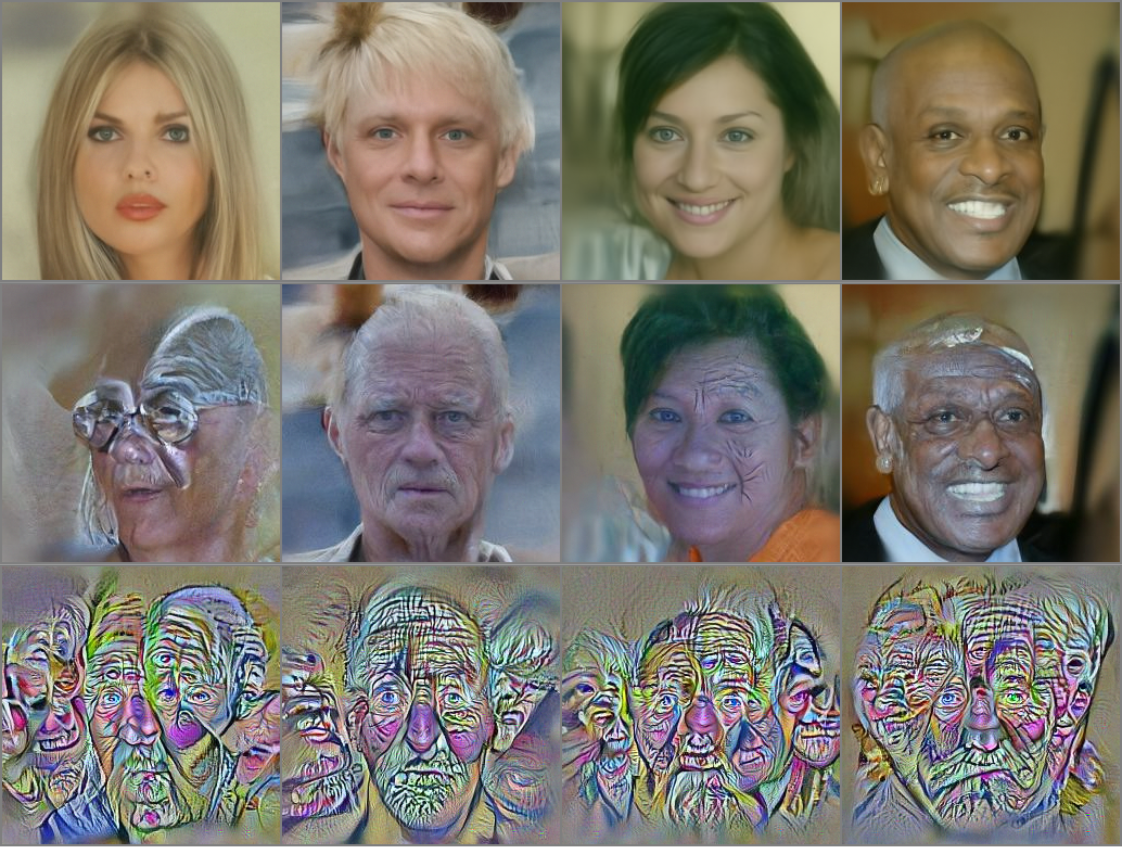
\includegraphics[scale=1.1]{ch2-diffusion-models/clip-guidance-experiment-3.png}
    \captionsetup{width=\textwidth} % set the width of the caption
    \caption{\textbf{CLIP Classifier Guidance.} The figure illustrates guiding
    image generation using a loss function that measures the distance between
    CLIP image embeddings $I_{t}$ and the text prompt reference $T_{t}$. The gradient information gives the direction that minimize the distance between the two embeddings. Using as prompt $\mathrm{y}=$``\texttt{old, senior, oldster, elderly, golden-ager}'' to generate images of people with hats with a guidance scale $\gamma=20$ at middle row. Last image is a failure mode when we use a higher guidance scale $\gamma=2000$ that breaks image semantic.}
    \label{fig:clip-guidance-old-experiment}
  \end{figure}

\begin{figure}[ht]
    \centering
    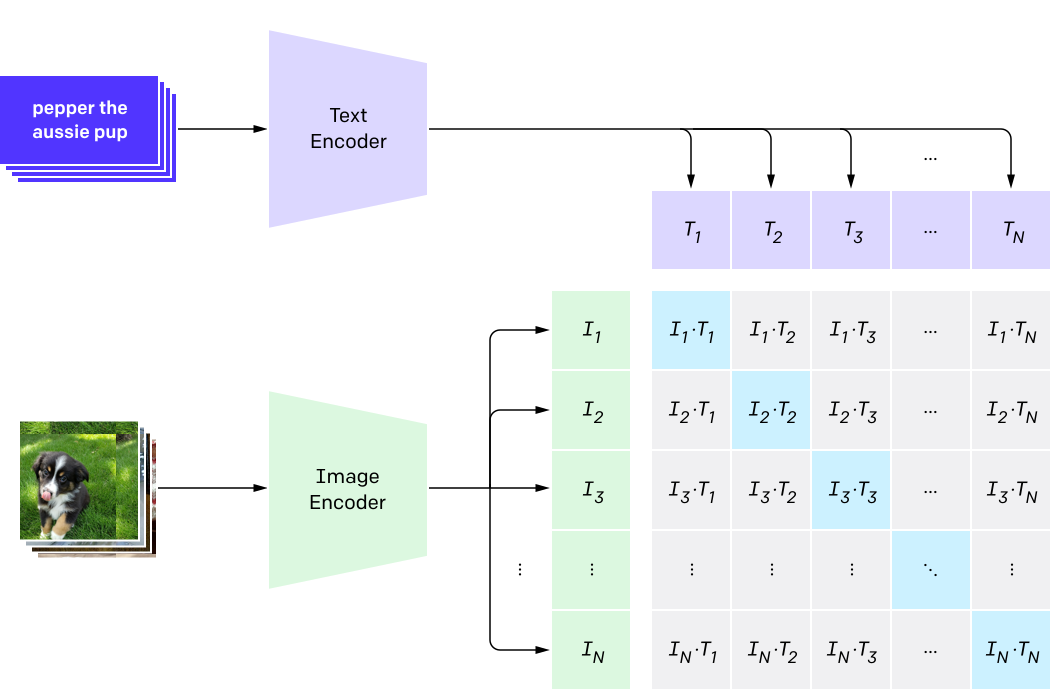
\includegraphics[scale=0.5]{ch2-diffusion-models/clip-overview-a.png}
    \captionsetup{width=\textwidth} % set the width of the caption
    \caption{\textbf{CLIP overview.} Text-to-image joint embedding space. \textbf{Source:} Learning Transferable Visual Models From Natural Language Supervision \citep{radford2021learning}.}
    \label{fig:clip-overview}
  \end{figure}

\noindent \textbf{Classifier Guidance with CLIP Embeddings}. Figure~\ref{fig:clip-guidance-old-experiment} illustrates an experiment using classifier guidance to control image generation. Specifically, the OpenAI CLIP model \cite{radford2021learning} guides a pretrained diffusion model (\href{https://huggingface.co/google/ddpm-celebahq-256}{google/ddpm-celebahq-256}) to generate
images of elderly people. The CLIP model includes an image encoder and a text encoder trained to match images with text descriptions (Figure~\ref{fig:clip-overview}). \\ 

\noindent First, we compute the text embedding $T_{\mathrm{y}}$ for the prompt $\mathrm{y}=$``\texttt{old, senior, oldster, elderly, golden-ager}'',  representing the desired image attribute. During sampling, we pass a denoised version of the steps $\hat{\mathrm{x}}_{t\rightarrow 0}$ (see Section~\ref{sec:DDIM}) to the CLIP image encoder to obtain an image embedding $I_{t}$. A loss function $\ell(I_{t}, T_{\mathrm{y}})$ measures the distance between these
embeddings at each timestep. Notice that $T_{\mathrm{y}}$ is fixed during the
whole sampling process, providing the gold standard for signal $\mathrm{y}$. We then backpropagate to obtain the gradient of the loss with respect to $\mathrm{x}_{t}$, $\nabla_{x}\log p_{\phi}(\mathrm{y}\mid \mathrm{x})$. \\

\noindent Using this conditional gradient, we guide the sampling proocess towards regions where the conditional log-likelihood is higher. By repeating this process throughout the Markovian steps, we can generate samples that match the prompt 
description. \\

\noindent \textbf{Limitations of Classifier Guidance.} Whle classifier guidance is powerful, it has limitations:

\begin{enumerate}
    \item The signal must come from a differentiable classifier, which is not always the case (e.g. decision trees or random forests are not compatible).
    \item The gradient must be computed at every denoising step, making it impractical for large models due to computational cost.
    \item Robust classifiers for noise are rare, limiting signal efectiveness, especially in the early steps where the sample is mostly noise. This limitation can be mitigated by using denoised versions of intermediate steps \cite{bansal2023universal}.
\end{enumerate}

\noindent Overall, while classifier guidance offers precise control over diffusion models,
these limitations must be considered.


\subsection{Classifier Free Guidance (CFG)}

\textbf{C}lassifier-\textbf{f}ree \textbf{G}uidance (CFG) is a technique for guiding diffusion models without using a separate classifier model \cite{Ho2022ClassifierFreeDG}. The key is to jointly train the unconditional and conditional model, introducing a null label $\emptyset$ that 
represent the unconditional model, without any signal effect. This means
that conditioning information is droupout during training with some percentage. When this happens, the conditional signal $\mathrm{y}$ is randomly discarded and replaced by $\emptyset$ with probability $p_{\text{uncond}}$ to trained the unconditional model. \\

\noindent During sampling, the output of the model is extrapolated in the diretion of
$\epsilon_{\theta}^{(t)}(\mathrm{x}_{t}\mid\mathrm{y})$ and away from
$\epsilon_{\theta}(\mathrm{x}_{t}\mid\emptyset)$ as follows: \\

\begin{equation}\label{eqn:cfg}
    \hat{\epsilon}_{\theta}^{(t)}(\mathrm{x}_{t}\mid\mathrm{y}) = \epsilon_{\theta}^{(t)}(\mathrm{x}_{t}\mid\emptyset) + \gamma \cdot (\epsilon_{\theta}^{(t)}(\mathrm{x}_{t}\mid\mathrm{y}) - \epsilon_{\theta}^{(t)}(\mathrm{x}_{t}\mid\emptyset))
\end{equation}


% \section{Enhancements \& Improvements}

% \ca{Paraphrase the following: Ho et al (2020) show how to derive $\mu_{\theta}$
% from the denoiser network $\epsilon_{\theta}^{(t)}$, and fix $\Sigma_{\theta}$ to a constant. In a follow-up work \cite{nichol2021improved} present a strategy
% for learning $\Sigma_{\theta}$, which enables the model to produce high quality
% samples with fewer diffusion steps...} \\

% \noindent A direct improvement to the DDPM was made in \cite{nichol2021improved}, in which they learn not only $\mu$ but also the variance $\sigma^{2}$ of the reverse process. This directly improves the likelihood estimation achieved by the model. \\

% \begin{figure}[ht]
%     \centering
%     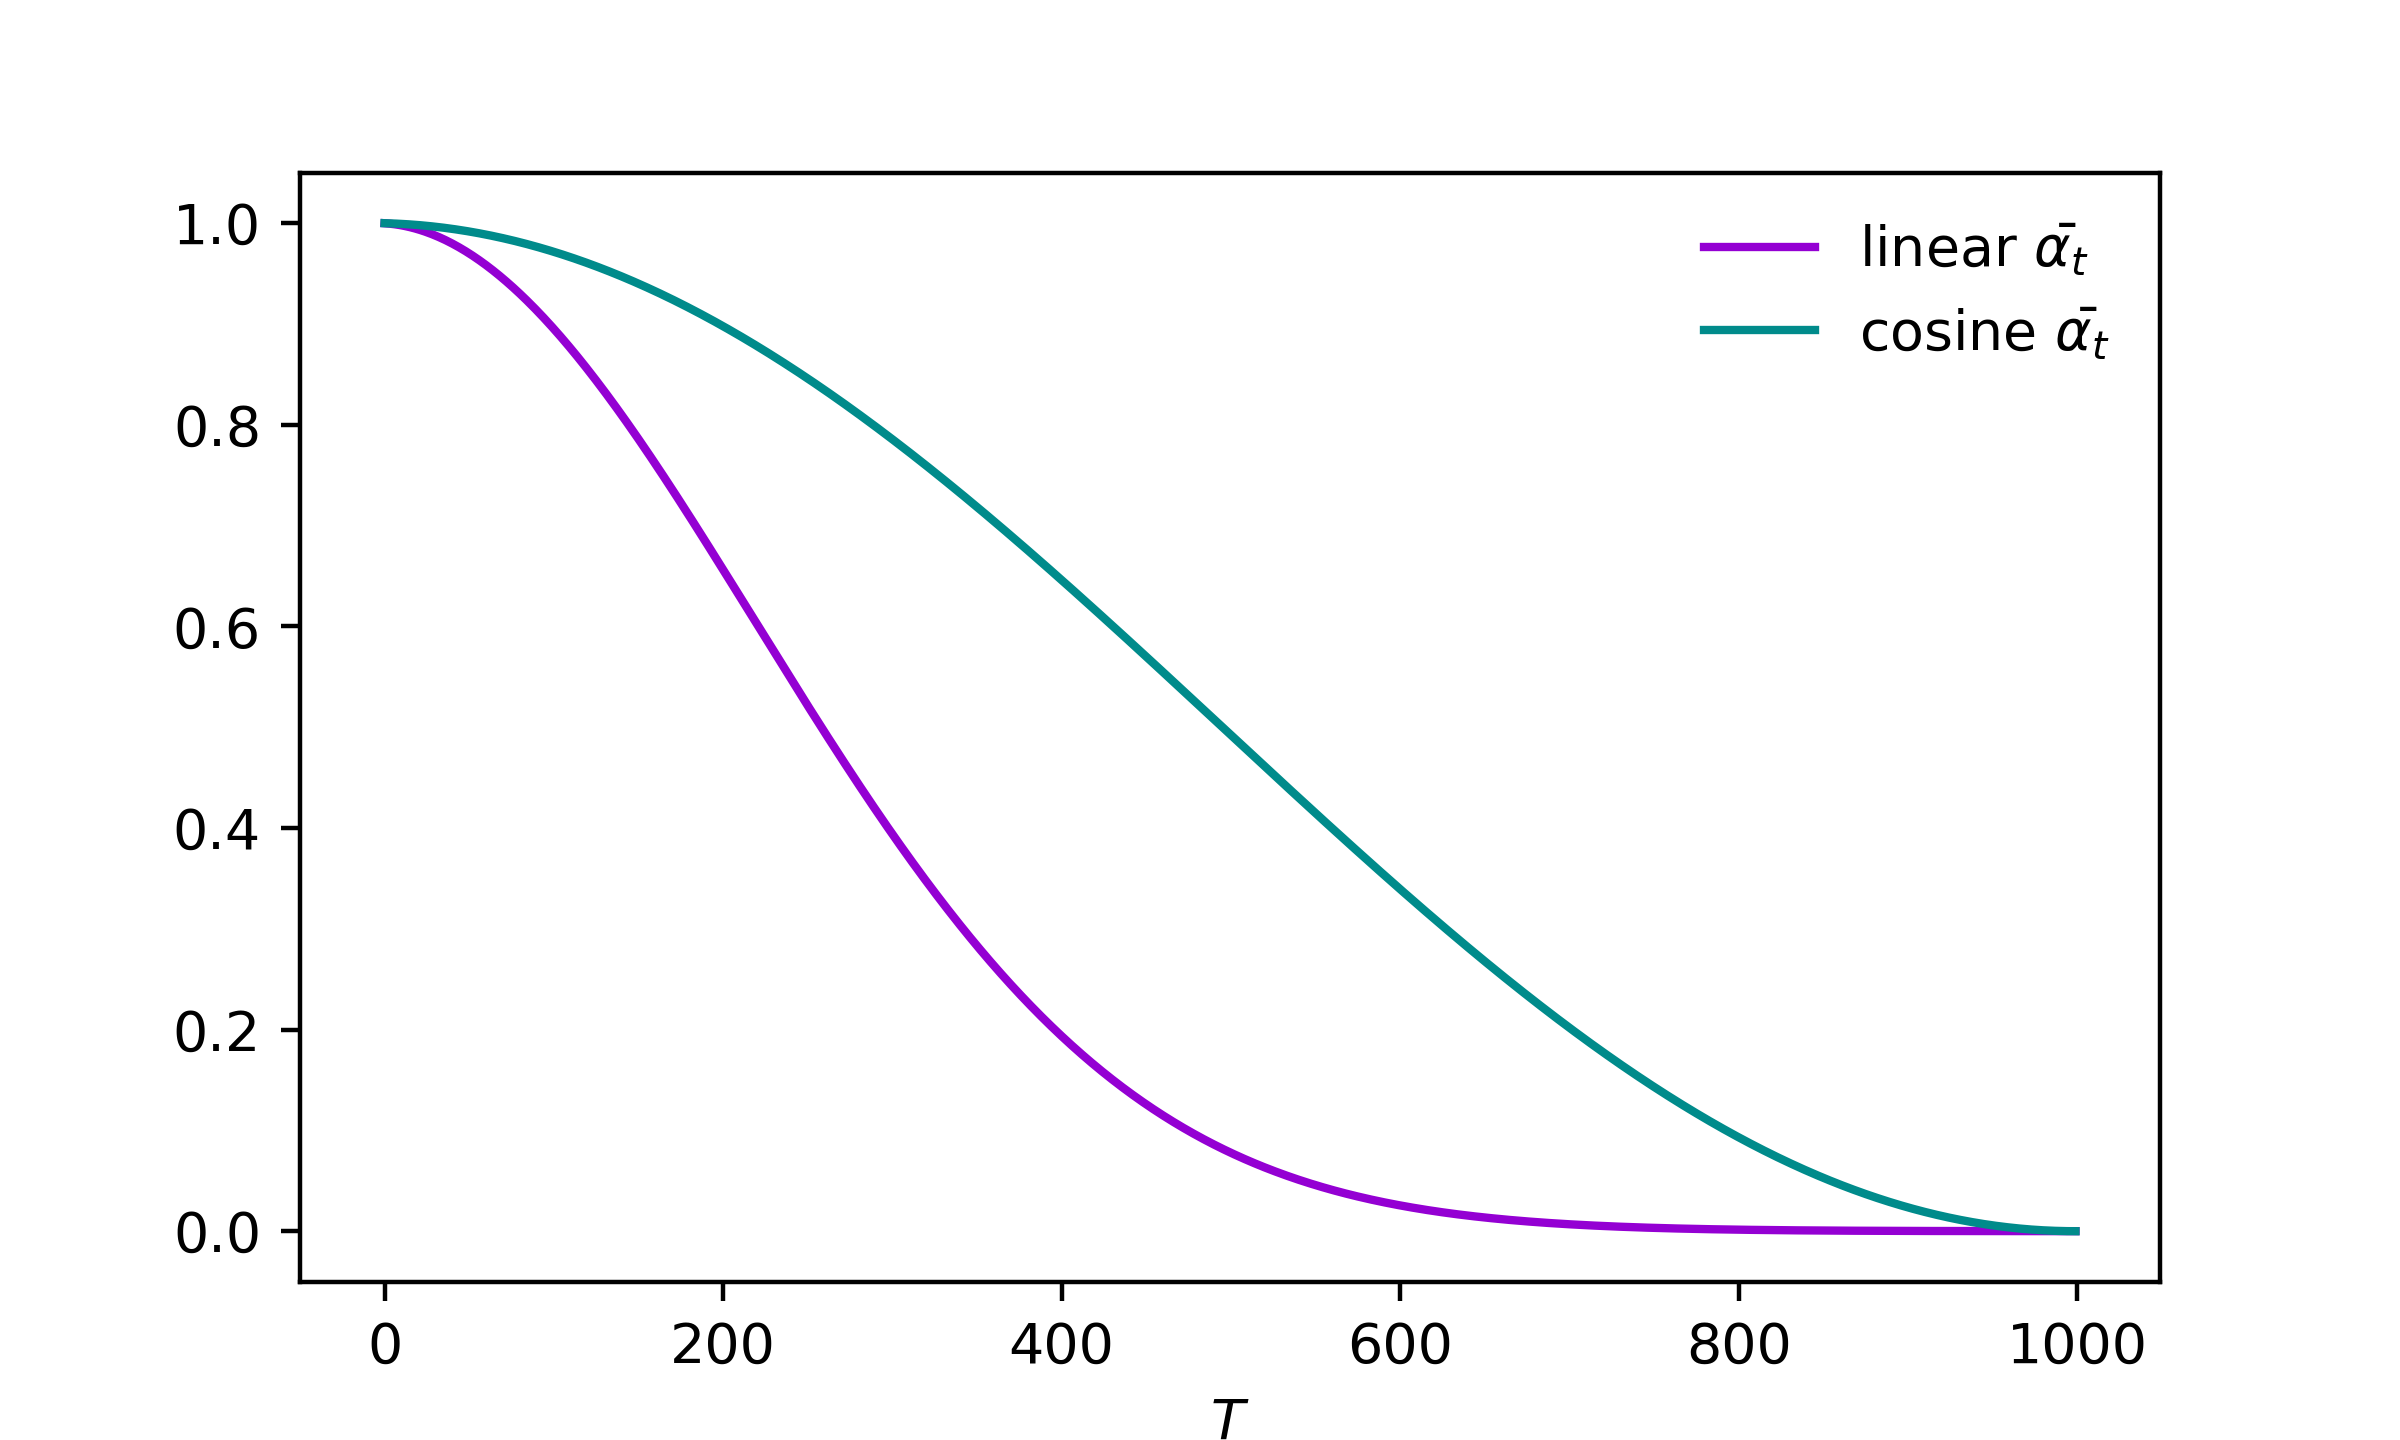
\includegraphics[scale=0.75]{ch2-diffusion-models/ddpm-linear-cosine-scheduler.png}
%     \captionsetup{width=\textwidth} % set the width of the caption
%     \caption{\textbf{Linear vs. Cosine scheduler} introduce in \cite{nichol2021improved}. Destroying the input structure smoothly is beneficial (regard what?) over using a simple linear scheduler \ca{esta figura suma realmente?}.}
%     \label{fig:ddpm-linear-vs-cosine-scheduler}
%   \end{figure}

% \noindent Regarding the variance scheduler, the same work found that the linear scheduler implemented in the DDPM paper was suboptimal because destroying the image very early in the backward chain left a lot of intermediate states redundant. Instead, a cosine scheduler was proposed, which gradually destroys the image structure, providing further informative steps to the denoiser as it shown in Figure~\ref{fig:ddpm-linear-vs-cosine-scheduler}. \\

% Notably, the work of \cite{rombach2022highresolution} in improving the model architecture and the training process to scale the resolution.

\section{Denoising Diffusion Implicit Models}\label{sec:DDIM}

% \ca{Simplificar esta sección, destacar más experimento realizado con imagen Pascal}. \\

\begin{figure}[t]
  \centering
  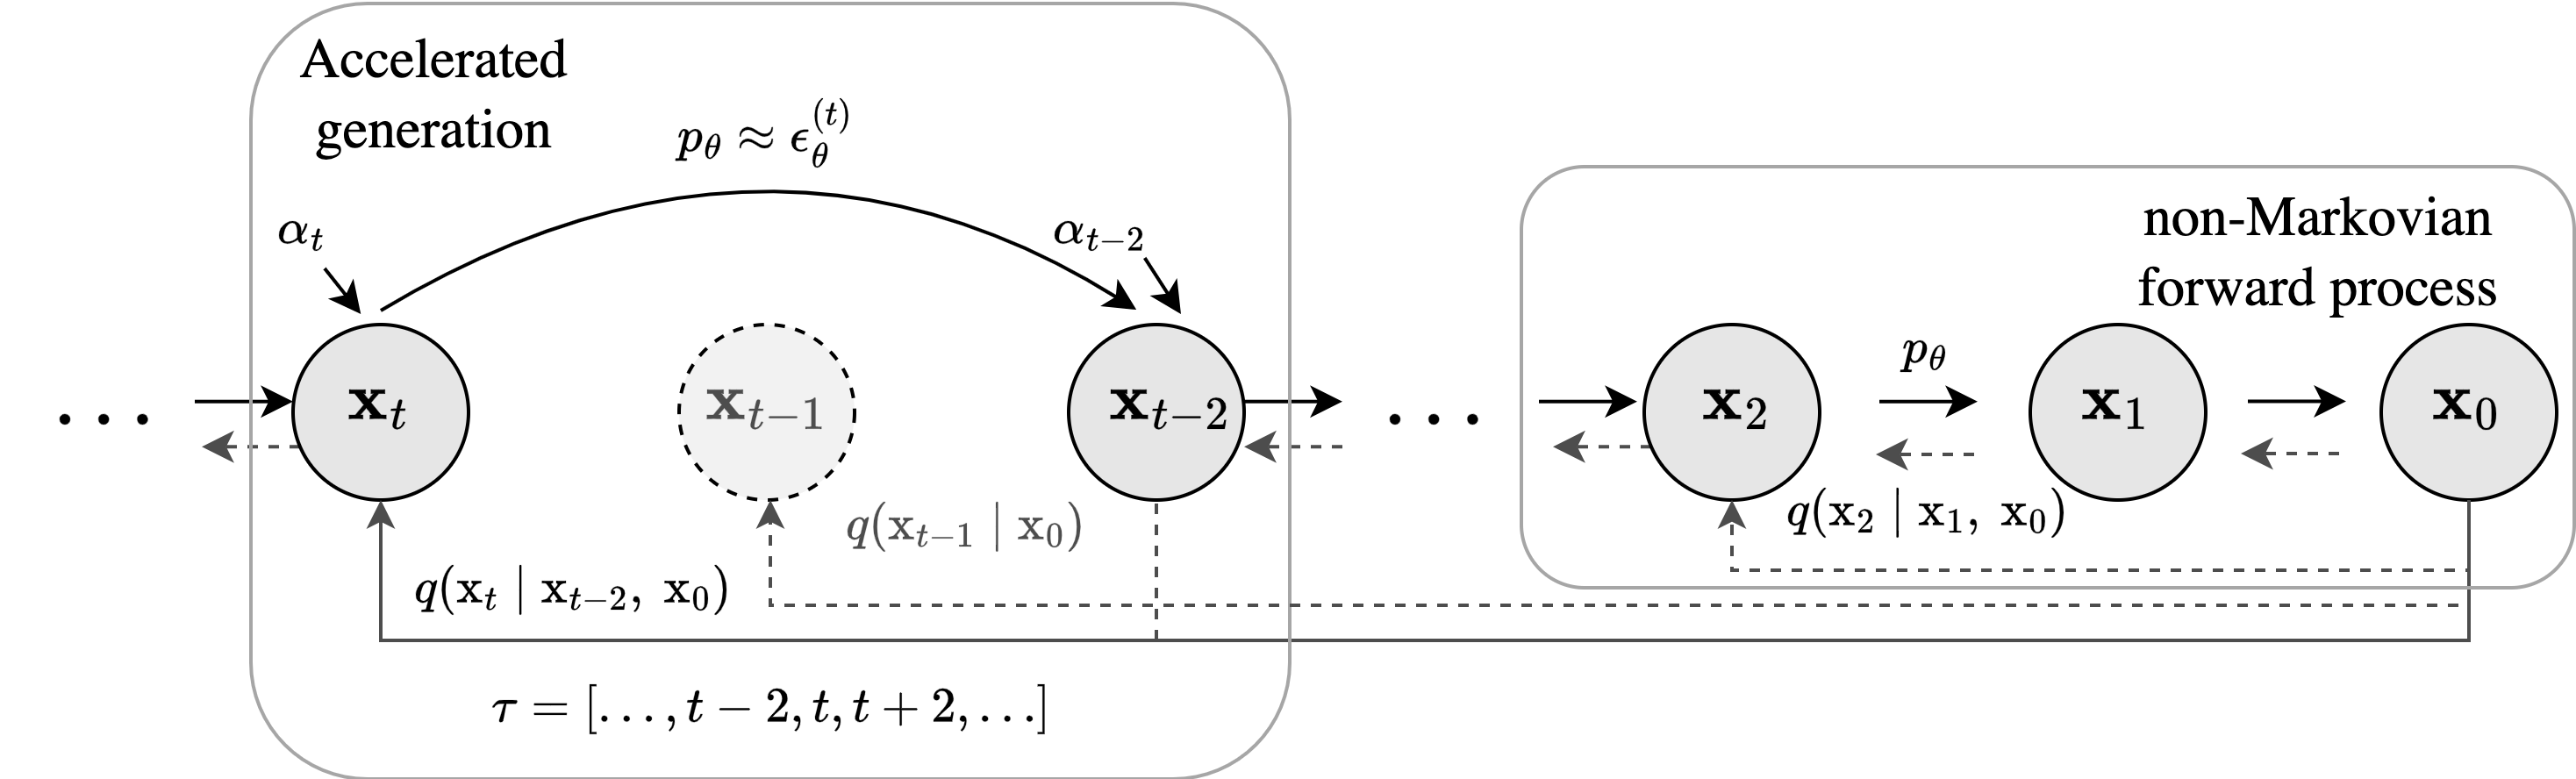
\includegraphics[scale=0.87]{ch2-diffusion-models/DDIM-no-markovian.png}
  \captionsetup{width=\textwidth} % set the width of the caption
  \caption{\textbf{DDIM non-Markovian forward process.} \textbf{Left:} Ilustration of accelerated generation skipping the uneven intermediate steps, the denoiser network $\epsilon_{\theta}^{(t)}$ predicts the amount of noise added to $\mathrm{x}_{t}$ from step $t-2$, instead $t$. \textbf{Right:} the non-Markovian graphical model.}
  \label{fig:ddim-non-markovian}
\end{figure}

The authors demonstrate that the DDPM forward process can be reformulated as a family of non-Markovian generative processes. Their resulting variational training objectives share a common surrogate objective, precisely aligning with the one used to train DDPM. This approach allows for the use of non-Markovian diffusion processes during inference with the pretrained DDPM model, leading to short generative Markov chains that can be sampled in just a few steps. Increasing the sample efficiency significantly but introducing a trade-off between sample quality.

% \noindent Usando regla de Bayes y forzando XYZ se obtiene la siguiente expresión para el forward process que describe un proceso no-Markoviano, ilustrado en la Figura~\ref{fig:ddim-non-markovian}:

\noindent Using Bayes rules we obtain the following expression for the non-Markovian forward process, illustrate in Figure~\ref{fig:ddim-non-markovian}:
\begin{equation}\label{eqn:ddim-non-markovian-marginal-eqn7}
    q_{\sigma}(\mathrm{x}_{t-1}\mid\mathrm{x}_{t}, \mathrm{x}_{0}) = \mathcal{N}(\sqrt{\alpha_{t-1}} \mathrm{x}_0 + \sqrt{1 - \alpha_{t-1} - \sigma_{t}^{2}}\cdot\frac{\mathrm{x}_{t} - \sqrt{\alpha_{t}}\mathrm{x}_{0}}{\sqrt{1-\alpha_{t}}}, \sigma_{t}^{2}I)
\end{equation}

% \noindent The backward process is...\\

\noindent \textbf{Prediction of noise-free observations.} We can obtain 
a denoised observation $\tilde{\mathrm{x}}_{t\rightarrow 0}$ from any arbitrary
intermediate state $\mathrm{x}_{t}$ by simple isolating $\mathrm{x}_{0}$ in Equation~\ref{eqn:reparameterization-trick} (Section~\ref{sec:reparameterization-trick})\footnote{In DDIM paper they use $\alpha_{t}=\alpha_{t} / \alpha_{t-1}$ to avoid using $\beta_{t}$, $\alpha_{t}$, and $\bar{\alpha}_{t}$ (See Appendix C.2 in \cite{song2020denoising})}. The caveat is that instead of sampling
 $\epsilon\sim\mathcal{N}(0, I)$,  we use the noise prediction given by the pretrained denoiser network $\epsilon_{\theta}^{(t)}$ at level $t$.

\begin{equation}\label{eqn:ddim-denoised-observation-eqn9}
    f_{\theta}^{(t)}(\mathrm{x}_{t}) = \frac{\mathrm{x}_{t} - \sqrt{1-\alpha_{t}}\epsilon_{\theta}^{(t)}(\mathrm{x}_{t})}{\sqrt{\alpha_{t}}} = \tilde{\mathrm{x}}_{t\rightarrow 0} 
\end{equation}

\noindent Then, by replacing Equation~\ref{eqn:ddim-denoised-observation-eqn9} in Equation~\ref{eqn:ddim-non-markovian-marginal-eqn7} we can compute $q_{\sigma}(\mathrm{x}_{t-1}\mid\mathrm{x}_{t}, f_{\theta}^{(t)}(\mathrm{x}_{t}))$ and sample $\mathrm{x}_{t-1}$ by:

\begin{equation}\label{eqn:ddim-sample-prev-xt-eqn12}
    \begin{split}
    \mathrm{x}_{t-1} &= \sqrt{\alpha_{t-1}}\mathrm{x}_{0} + \sqrt{1-\alpha_{t-1}-\sigma_{t}^{2}}\cdot\frac{\mathrm{x}_{t} - \sqrt{\alpha_{t}}\mathrm{x}_{0}}{\sqrt{1-\alpha_{t}}} + \sigma_{t}\epsilon_{t} \\ 
    \mathrm{x}_{t-1} &= \sqrt{\alpha_{t-1}}\bigg(\frac{\mathrm{x}_{t} - \sqrt{1 - \alpha_{t}}\epsilon_{\theta}^{(t)}(\mathrm{x}_{t})}{\sqrt{\alpha_{t}}}\bigg) + \sqrt{1 - \alpha_{t-1} - \sigma_{t}^{2}} \\ &~~~~ \cdot\frac{\textcolor{red}{\cancel{\mathrm{x}_{t}}} - \textcolor{teal}{\cancel{\sqrt{\alpha_t}}}((\textcolor{red}{\cancel{\mathrm{x}_{t}}}-\textcolor{blue}{\cancel{\sqrt{1-\alpha_{t}}}}\epsilon_{\theta}^{(t)}(\mathrm{x}_{t})) / \textcolor{teal}{\cancel{\sqrt{\alpha_{t}}}})}{\textcolor{blue}{\cancel{\sqrt{1-\alpha_{t}}}}} + \sigma_{t}\epsilon_{t} \\
    \mathrm{x}_{t-1} &= 
    \sqrt{\alpha_{t-1}}\underbrace{\bigg(\frac{\mathrm{x}_{t}-\sqrt{1-\alpha_{t}}\epsilon_{\theta}^{(t)}(\mathrm{x}_{t})}{\sqrt{\alpha_{t}}}\bigg)}_{\text{``predicted $\mathrm{x}_{0}$''}} 
    + \underbrace{\sqrt{1-\alpha_{t-1} - \sigma^2_{t}}~\cdot~\epsilon_{\theta}^{(t)}(\mathrm{x}_{t})}_{\text{``direction pointing to $\mathrm{x}_{t}$''}}
    + \underbrace{\sigma_{t}\epsilon_{t}}_{\text{random noise}}
    \end{split}
\end{equation}

\noindent \textbf{Multiple generative processes} are contain in Equation~\ref{eqn:ddim-sample-prev-xt-eqn12} depending of $\sigma$ election. Again,
the main takeaway is that all share the same surrogate objective with DDPM, 
it is possible to use the same denoiser model $\epsilon_{\theta}^{(t)}$ without any additional training for different inference processes. The stochasticity comes from $\epsilon_{t}\sim\mathcal{N}(0,, I)$, a Gaussian noise independent of $\mathrm{x}_{t-1}$, and modulate by the noise scheduler. \\

\begin{enumerate}
    \item The generative process, obtained by reversing Markovian forward process in DDPM, can be derived from Equation~\ref{eqn:ddim-sample-prev-xt-eqn12} by using $\sigma_{t} = \sqrt{(1-\alpha_{t-1}) / (1 - \alpha_{t})}\sqrt{1-\alpha_{t}/\alpha_{t-1}}$ for all $t$.
    \item A deterministic forward process arise when $\sigma_{t}=0$, for all $t$, except for the initial noise. The authors names this specific generative process as denoising diffusion implicit models (DDIM).
\end{enumerate}

\noindent \textbf{Accelerate inference.} With the possiblity to design non-Markovian forward process using the same pretrained model of DDPM, the authors propose to accelerate the inference process by skipping intermediate steps. Subset of latent variables $\{\mathrm{x}_{\tau_1}, \dots, \mathrm{x}_{\tau_{s}} \}$ where $\tau$ is an increasing subset sequence of $[1, \dots, T]$ , of length $S$. We define a forward process over the subset such that $q(\mathrm{x}_{\tau_i}\mid\mathrm{x}_{0})=\mathcal{N}(\sqrt{\alpha_{\tau_{i}}}\mathrm{x}_{0}, (1-\alpha_{\tau_{i}})I)$ matches the marginals, see left part of the Figure~\ref{fig:ddim-non-markovian}. Therefore, we can accelerate the inference increasing the number of steps between the sequence subset, and introducing a trade-off between sample quality and computational cost in doing so. \\

\noindent Introducing the hyperparameter $\eta\in\mathbb{R}^{+}$ for control the
sampling stochasticity from DDIM ($\eta=0$) to DDPM ($\eta=1$) in Equation~\ref{eqn:ddim-sample-prev-xt-eqn12}, and use subsequence $\tau$ of different length 
for control the sample aceeleration.
\begin{equation}\label{eqn:ddim-to-ddpm-variance}
    \sigma_{\tau_{i}}(\eta) = \eta \sqrt{(1-\alpha_{\tau_{i-1}}) / (1-\alpha_{\tau_{i}})}\sqrt{1-\alpha_{\tau_{i}}/\alpha_{\tau_{i-1}}}
\end{equation}
It is possible to produce samples with a similar quality of DDPM $1000$ steps using $20-100$ DDIM steps by measuring the quality with the Fréchet inception distance (FID). This means a speed ups of $10\times$ to $100\times$ over DDPM generation process \cite{song2020denoising}. In practice, DDIM is commonly used as a sampler and an efficient way to accelerate the sampling process, as utilized in this thesis. \\

% \ca{Acá hablar dela propiedaded de consistencia y explorar el espacio latente interviniendolo} 

\noindent \textbf{Sample consistency with DDIM.} As a consequence of the deterministic forward process, we have \textit{\textbf{sample consistency}}. Given any arbitrary length $\tau$, the image generated from the initial sample step $\mathrm{x}_{T}$ are fairly similar, in the authors words ``it would appear that $\mathrm{x}_{T}$ alone would be an informative latent encoding of the image''.  Hence, they suggest that high level features of the images $\mathrm{x}_{0}$ are determined by the initial sample step $\mathrm{x}_{T}$. \\

\noindent The sample consistency property can be useful for inverse problems. For instance, in Figure~\ref{fig:ddim-inversion-pascal}, given an input image (Pedro Pascal face) we can estimate the initial noise $\tilde{\mathrm{x}}_{t}$, and run the generative process to recover the input. However, the input is not perfectly recovered, the reason could be:

\begin{itemize}
    \item It is interesting that high level features are encoded by $\mathrm{x}_{T}$ and doesn't vary as long as increase the number of steps to generate the final sample. However, the quality is better as long as the length of the trajectory increase. Therefore, a trick to obtain a recovered input with higher fidelity is to skip the first steps and start the denoising process from there, avoiding higher feature modification.
    \item The estimation error is illustrate as a trade-off between denoising from the first step that conserve face semantic but change higher features and skipping a set of denoiser steps conserving semantic but with lower quality.
    \item External input not generated by the model are not guarantee to be recover given the generative capacities of $\epsilon_{\theta}$. In the illustration, the input is external but is the generative process is perform by a DDPM trained model on a dataset of celebrities faces.
\end{itemize}

% \noindent Interesting is that high level features are encoded by $\mathrm{x}_{T}$ and doesn't vary as long as increase the number of steps to generate the final sample. However, the quality is better as long as the length of the trajectory increase. \\

\begin{figure}[ht]
    \centering
    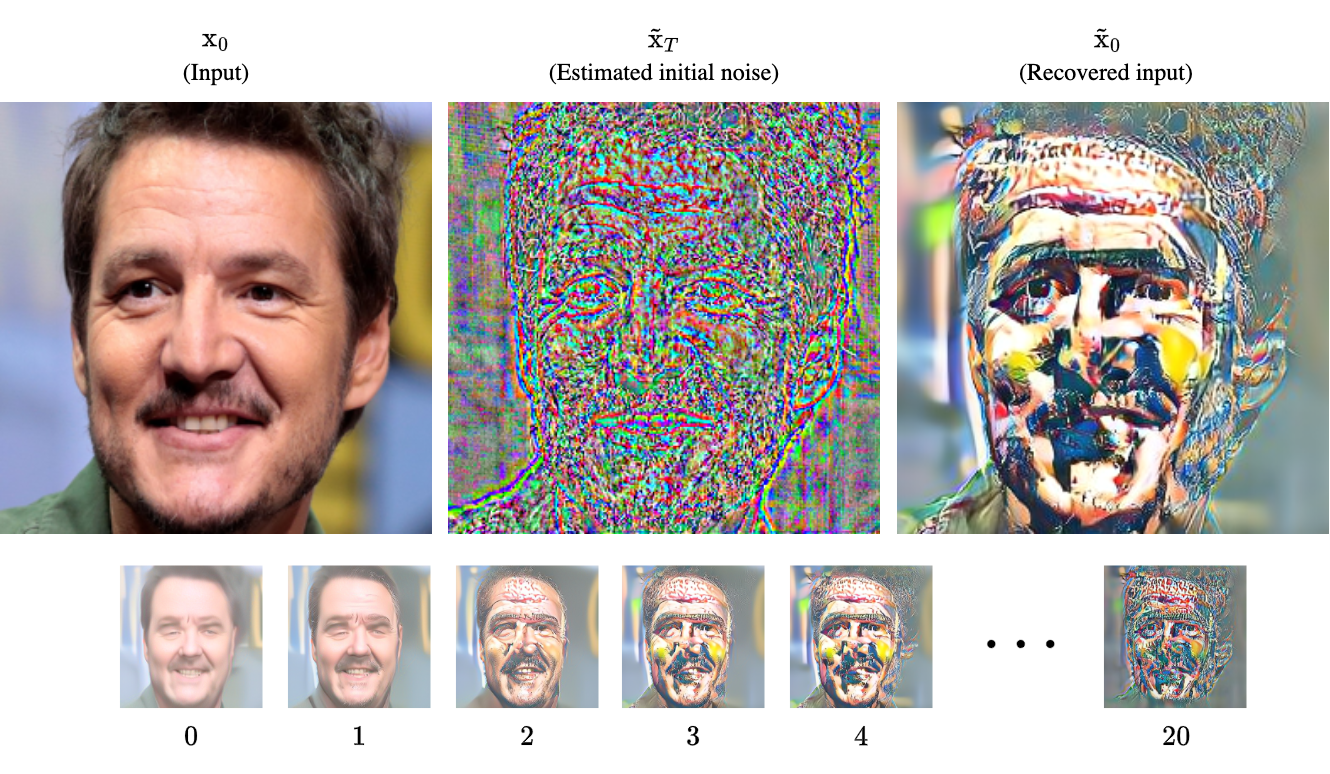
\includegraphics[scale=0.75]{ch2-diffusion-models/DDIM_Inversion_Pascal_2.png}
    \captionsetup{width=\textwidth} % set the width of the caption
    \caption{\textbf{DDIM inversion example using $50$ inference steps.} A Pedro Pascal photo to estimate the initial noise $\tilde{\mathrm{x}}_T$ using DDIM with the pretrained model \texttt{google/ddpm-celebahq-256} on the celebrity faces dataset CelebaHQ. Then, the input si reconstructed using the estimated noise as starter point. Below images are different results skpping the first $n$ inference steps of the denoising process.}
    \label{fig:ddim-inversion-pascal}
  \end{figure}

\section{Summary}

In summary, a typical diffusion model framework can be implemented as follows:\\

\noindent A \textbf{forward process} that consists of a Markovian chain of states $\{\mathrm{x}\}_{0:T}$ that takes the original image $\mathrm{x}_0$ and iteratively adds noise until getting isotropic Gaussian noise $\mathrm{x}_{T}$. \\

\noindent In the reverse, or \textbf{backward process}, a model learns how to gradually remove the noise to recover the data structure. In most implementations model this denoising endeavour using some U-net neural network architecture with attention modules. \\

\noindent The sequence of intermediate states provides a detailed roadmap when destroying the observation such as images and leaves a trail to the denoiser network to recover the input structure. Therefore, the forward process acts in a \textbf{self-supervised} manner generating the labels for the data itself. \\

\noindent It is possible to use a model to predict the noisy image directly, or indirectly via predicting the noise, and then substracting from the state. Nevertheless, \textbf{the core idea of the training objective is to reduce the error between the noise prediction and the true noise} used to destroy the sample at a given step. \\

\noindent The noise used to destroy the structure in data is carefully handled by a deterministic function called \textbf{noise scheduler}. It determines the variance schedule, $\beta_{1}, \dots, \beta_{T}$, or the specific amount of noise injected in each timestamp $t$ during the Markovian chain. \\

\noindent Finally, we have a model that can \textbf{generate novel samples} from the data distribution \textbf{by sampling from a standard normal distribution and then 
successively remove noise}.
